\chapter{Methods}\label{chp:methods}
This Chapter aims to present some theoretical background for understanding the subsequent Chapters of the thesis. We define in more detail concepts and approaches previously mentioned in the introductory Chapter~\ref{chp:intro} like intransitivity and macroecological patterns. To start with, we present some basic concepts in networks theory in Section~\ref{chp:methods:networks}, as they will be used for studying both ecological and social systems in the first three Chapters. Once all the necessary networks' machinery is introduced, the Chapter digs into the particularities of ecological networks (Section~\ref{chp:methods:econet}) and defines mathematical models for studying ecological interactions (Section~\ref{chp:methods:ecointeract}). Although the presentation of this latter Section will be oriented toward ecological systems, the same concepts will be also applied to the study of social systems. Furthermore, to create a foundation for the part of the thesis that revolves around these social systems, Section~\ref{chp:methods:CSS} introduces some important concepts in computational social science and its challenges. Finally, Section~\ref{chp:methods:macro} explains the importance of finding patterns both in ecological and social systems.  \\

\section{Complex networks}\label{chp:methods:networks}
%\epigraph{In ecology—a world of vast and wildly complex connections—network theory has risen to play a significant research role and is undoubtedly here to stay.}{\textit{Theoretical Ecology 4th edition \cite{intro2020theoretical}}}
\epigraph{Why is network anatomy so important to characterize? Because structure always affects function.}{\textit{Steven Strogatz} \cite{strogatz2001exploring}}
%... i.e. evaluate emergent network-level properties and at the same time consider the behavior and functional role of nodes.
 %In any study of evolutionary ecology, food relations appear as one of the most important aspects of the system of animate nature. There is quite obviously much more to living communities than raw dictum ''eat or be eaten'', but in order to understand the higher intricacies of any ecological system, it is most easy to start from this crudely simple point of view. \cite{hutchinson1959homage}


 A network (or graph) is a mathematical structure 
 $G = (V, E)$, which consists of a set $V$ of elements called nodes and a set $E$ of links that connect pairs of nodes. A network is usually represented by its adjacency matrix $A$, a square matrix whose entries are:
 \begin{align*}
       A_{ij} &= 1 \, \,  \textrm{ if there is a link between nodes } \, i \, \textrm{ and } \, j , \\
       A_{ij} &= 0 \, \, \textrm{otherwise}.
 \end{align*}

For example, in Figure~\ref{fig:simpleNetwork}, we have the adjacency matrix of a simple network. This network represents the most basic scenario, in which nodes are all indistinguishable, and links  encode the existence of an interaction. To describe more complex circumstances, we can add more information to the links in at least three ways: with sign, weight, and direction. By including the sign of interactions (Figure~\ref{chp:methods:fig:adjacencies}a), one can discern the effect of the interaction on the nodes. Going further and introducing weighted links (Figure~\ref{chp:methods:fig:adjacencies}b), the interactions not only exist but also have a relative strength. Weight captures the fact that not all interactions are equally important. Finally, connections may exhibit directionality, making a difference between whether the relation is from node $i$ to node $j$ or vice versa.\\

\begin{figure}[h]
    \centering
    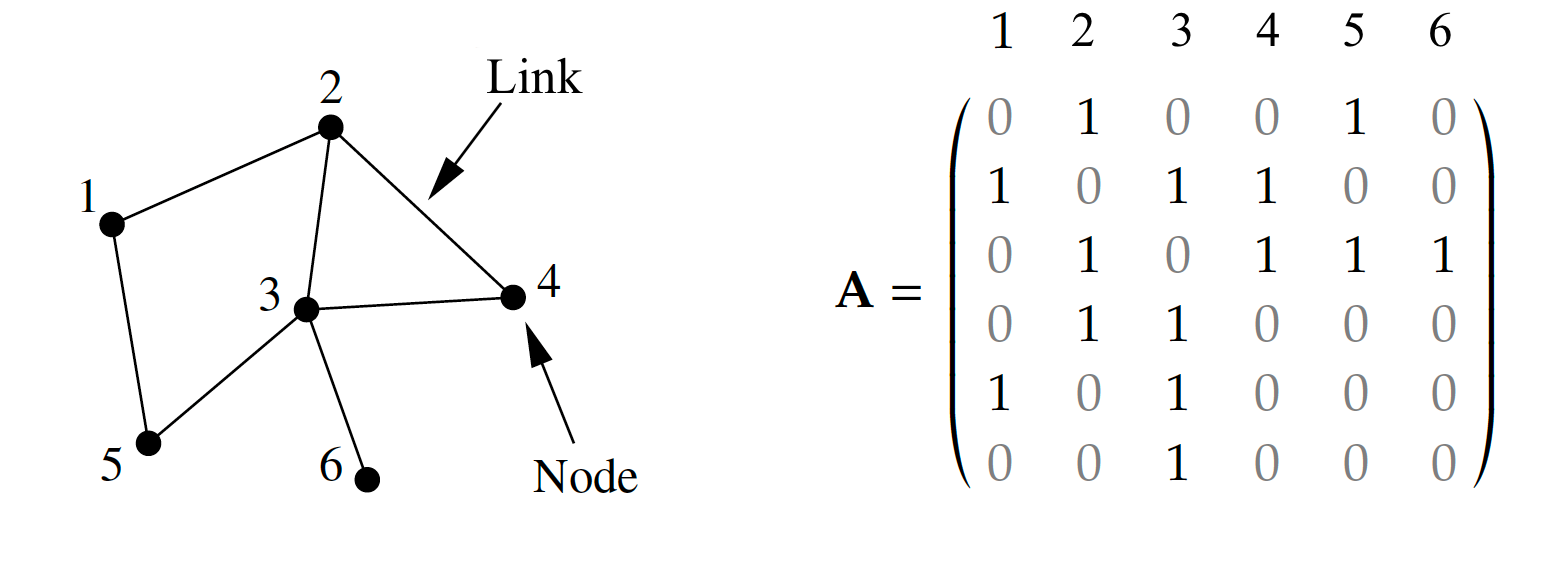
\includegraphics[width= 0.8\columnwidth]{figures/methods/fig_simpleNetwork.png}
    \caption[A simple graph]{A simple graph with its corresponding adjacency matrix. The diagonal elements must be zero for a network like this one with no self-edges, and the matrix must also be symmetric as every link between node $i$ and $j$ also exists between $j$ and $i$. Figure adapted from \cite{Newman2010}.}
    \label{fig:simpleNetwork}
\end{figure}

%Once presented with the formalism of graphs, we are ready to introduce the two most fundamental questions in network science: what does a node represent and when are two nodes connected? Trivial as they may seem, these questions are crucial to correctly describe a network according to a research question \cite{torres2021and}. In fact, networks are grouped in classes based on what their nodes represent --technological, transportation, economic, social, and biological/ecological \cite{Newman2010}. For our purposes, we will represent social and ecological systems as networks whose nodes are either agents of online social platforms (users and hashtags), species, or spatial locations in ecosystems. For example, in a food web, predator-prey interactions may be weighted to indicate the total energy flow between  predator and prey. Since, the energy flows from prey to predator, so a directed representation could also be used. In a social network, weighted connections may  represent the contact frequency between actors, and their sign may indicate friendship ($+$) or enmity ($-$). \\

Knowing which nodes are connected in a network provides, in principle, a comprehensive understanding of its structure. Nonetheless, interpreting raw network data can be challenging, which is why mathematical measures are defined to condense structural aspects quantitatively. Over the years, numerous measures have been defined. 
%including the degree $k$, the number of nodes connected to a node. 
In Appendix~\ref{chp:methods:predictors} we present a comprehensive list topological measures utilized in this thesis.

Finally, for the aim of this thesis, it is worth discussing bipartite networks. They are networks with two classes of nodes (or guilds in the ecological literature), and links connect only nodes of different classes. Bipartite networks commonly represent the membership of a set of species or people in groups of some kind. For example, we can represent pollination as a bipartite network in which the two guilds of nodes are plants and pollinators (regardless of taxa), and the links connect plants to their pollinators. To describe this mutualistic community, there is in principle no necessity for links that directly connect plants to other plants, or pollinators to other pollinators; the links in the bipartite network only run between nodes of different guilds. Therefore, if we group together all nodes of the same guild in the adjacency representation of the bipartite network, the diagonal blocks will be empty (Figure~\ref{chp:methods:fig:adjacencies}c).

\begin{figure}[t]
     \centering
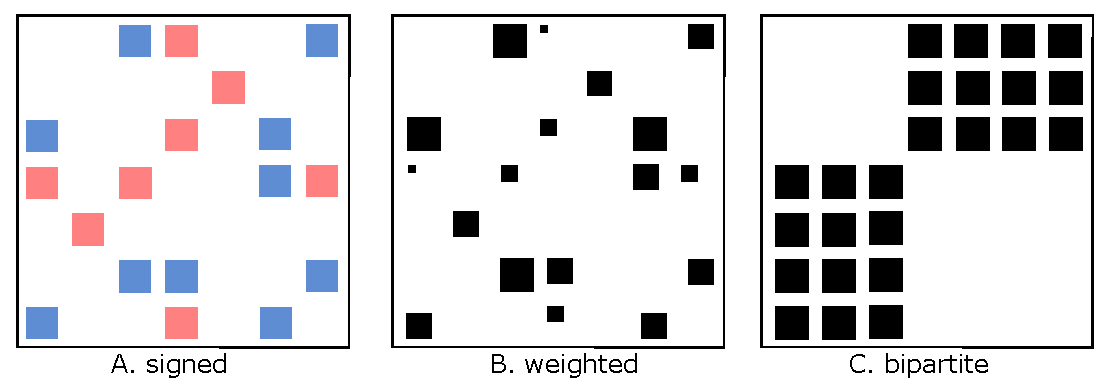
\includegraphics[width=\columnwidth]{figures/methods/fig_adjacencies.pdf}
 \caption[Adjacency matrices]{Adjacency matrices of several types of networks. Nodes are represented along the rows and columns. A square denotes the presence of an interaction, and its color and size represent the sign and weight, respectively. }
\label{chp:methods:fig:adjacencies}
\end{figure}

\subsection{Network models}

Network models suggest and explain the mechanisms behind node connection. All of these models have a similar approach: they eliminate unnecessary details and assume that links are set in a specific way. For example, just at random or according to some metrics. We may use models to reveal the circumstances in which our findings are valid and to understand the effects of the constraints that exist in the real world.

\paragraph{2D square lattice:} This model is not actually a \textit{complex} network, but a very ordered network since its nodes are discretely and consistently spaced from one another on the unit square. The eight adjacent nodes of a given node are thought to be their closest neighbors. The second closest nodes are the neighbors' neighbors, creating a total neighborhood of $24$ nodes.  This configuration can be thought of as a chessboard. The (discrete) distance between two nodes on a chessboard is the minimum number of moves that the king needs to move between them. In a more precise language, this definition of neighborhood is called Moore neighborhood and the distances between nodes are measured according to the Chebyshev distance. 2D lattices will be used in Chapter~\ref{chp:1} to represent a highly structured space.

\paragraph{Erd{\H{o}}s-R{\'e}nyi graph (ER):}  One of the most studied network models is the Erd{\H{o}}s-R{\'e}nyi  model \cite{erdos1959random}, where pairs of nodes are connected at random according to a fixed linkage probability $p$. It is used  as a null model in Chapters~\ref{chp:1} and \ref{chp:2} because it represents the simplest model for random graphs.

\paragraph{Random geometric graph (RGG):} 
In general, the random geometric graph is created by assigning a random location to its nodes by a predetermined probability distribution, and connecting two nodes by a link only if their distance falls within a predetermined distance, defined in a metric space \cite{Dall2002RandomGraphs}. For our purposes, nodes are randomly uniformly placed in the unit square and linked together according to the Euclidean distance.

\paragraph{Scale-free networks:} Our next step in complexity is to simulate scale-free networks. In particular, we employed the Barabasi-Albert model \cite{Albert2002StatisticalNetworks}. A network growth model based on preferential attachment where each new node is randomly connected to $m$ existing nodes with a probability proportional to the number of links that they already have.  To add up more realism, we use the Holme-Kim model \cite{Holme2002GrowingClustering}, which is a variant of a scale-free network and it can generate networks with a finite clustering coefficient. Both models are used in Chapter~\ref{chp:2}.

\paragraph{Network reshuffling:}
In the context of network theory, null models are
used to check whether a certain property of
a target network is just a consequence of chance, or
is due to a driving mechanism \cite{Newman2010}. The property can be
any macroscopic structure (e.g. nestedness in mutualistic
systems \cite{bastolla2009mutualism}), or a particular behavior of the underlying
dynamics (amplification of selection for advantageous mutants \cite{lieberman2005evolutionary}). The driving
mechanism to uncover can be the way in with the network is constructed (e.g. by an optimization process \cite{bastolla2009mutualism})
or the topological structure of the network (e.g. scale-free networks \cite{lieberman2005evolutionary}).\\

The modus operandi usually involves generating
randomizations of the original network where
some constraints are kept. Then, the property
will be evaluated in these networks and compared
against the original network.\\

We have already mentioned null models when presenting the ER
graph. This graph serves as a null model because it can
generate random networks with the same number of
nodes and average degree as the target network. If a
property of the original network does not depend on how
nodes connect, then the ensemble of ER networks, whose nodes
are linked at random, will also present that property. \\

Sometimes ER graphs are too disruptive
as null model since they dilute any trace of
structure. More conservative alternatives include
reshuffling the links and the weights of the original network. When reshuffling, links are interchanged among nodes
following certain rules. In particular, we
perform a reshuffling of each block
of bipartite networks in Section~\ref{chp:2:3:4}.
Those randomizations will be generated
through a Bernoulli process,
where a link between nodes $i$ and $j$ is created with probability
\begin{equation}
    P_{ij} = \frac{k_{i} + k_{j}}{2n},
\end{equation}
where $n$ is the total number of nodes, and $k_{i,j}$ is the degree of the original network.
This method conserves the connectance and the expected number of interactions of each node alone \cite{BiMat}. \\

Another reshuffling or rewiring is made in Section~\ref{chp3:1.3} as proposed in \cite{suweis2013emergence}, where links are interchanged according to a probability that depends on the degree and an external node property called \textit{niche}, which will be defined in Section~\ref{chp:methods:ecointeract}.

\section{Ecological networks}\label{chp:methods:econet}
\epigraph{Networks are particularly attractive to ecologists for providing a dynamic viewpoint from where scientists can simultaneously “see the forest and the trees”.}{\textit{Heleno et al.} \cite{heleno2014ecological}}
Once we have defined complex networks in general, we are ready to explore the role of networks in ecology. Depending on what nodes and links symbolize, we can divide ecological networks into two categories: interaction networks and spatial networks. %Nevertheless, this classification is highly biased toward the objective of this thesis. One could group networks across levels of organization, and would obtain a hierarchy of networks: individual-based networks, followed by species-based, and finally, clade-based networks \cite{guimaraes2020structure}.
One ecosystem may well be represented by these two categories simultaneously since a network is just a partial representation of one aspect of a complex system \cite{strogatz2001exploring}. Each type possesses attributes that make it suitable for dealing with certain questions.\\


%Chapter Structured interactions = space-based
%Chapter Structured predictors  and quantifiers = species-based

\subsection{Interaction networks}

Interaction networks are the most widely used networks in ecology \cite{kefi2020theoretical}. Nodes represent species and links are interactions between them. There are many well-documented types of interactions among species, so there are many types of networks depending on the interaction they describe. For instance, food webs are directed networks  of who eats whom, (Figure~\ref{chp:methods:fig:history}a). Ecological network research has been mainly focused  on food webs \cite{pascual2006ecological}, even if Darwin had already described the now-classic \textit{entangled bank} back in 1859, suggesting that species are ``dependent on each other in so complex a manner'' \cite{darwin1859origin}. There is a great variety of non-trophic interactions such as ecosystem engineering, facilitation, or antagonism \cite{kefi2012more}. Even more, there are interactions with  both trophic as well as non-trophic components, like pollination and seed dispersal.\\

\begin{figure}
    \centering
    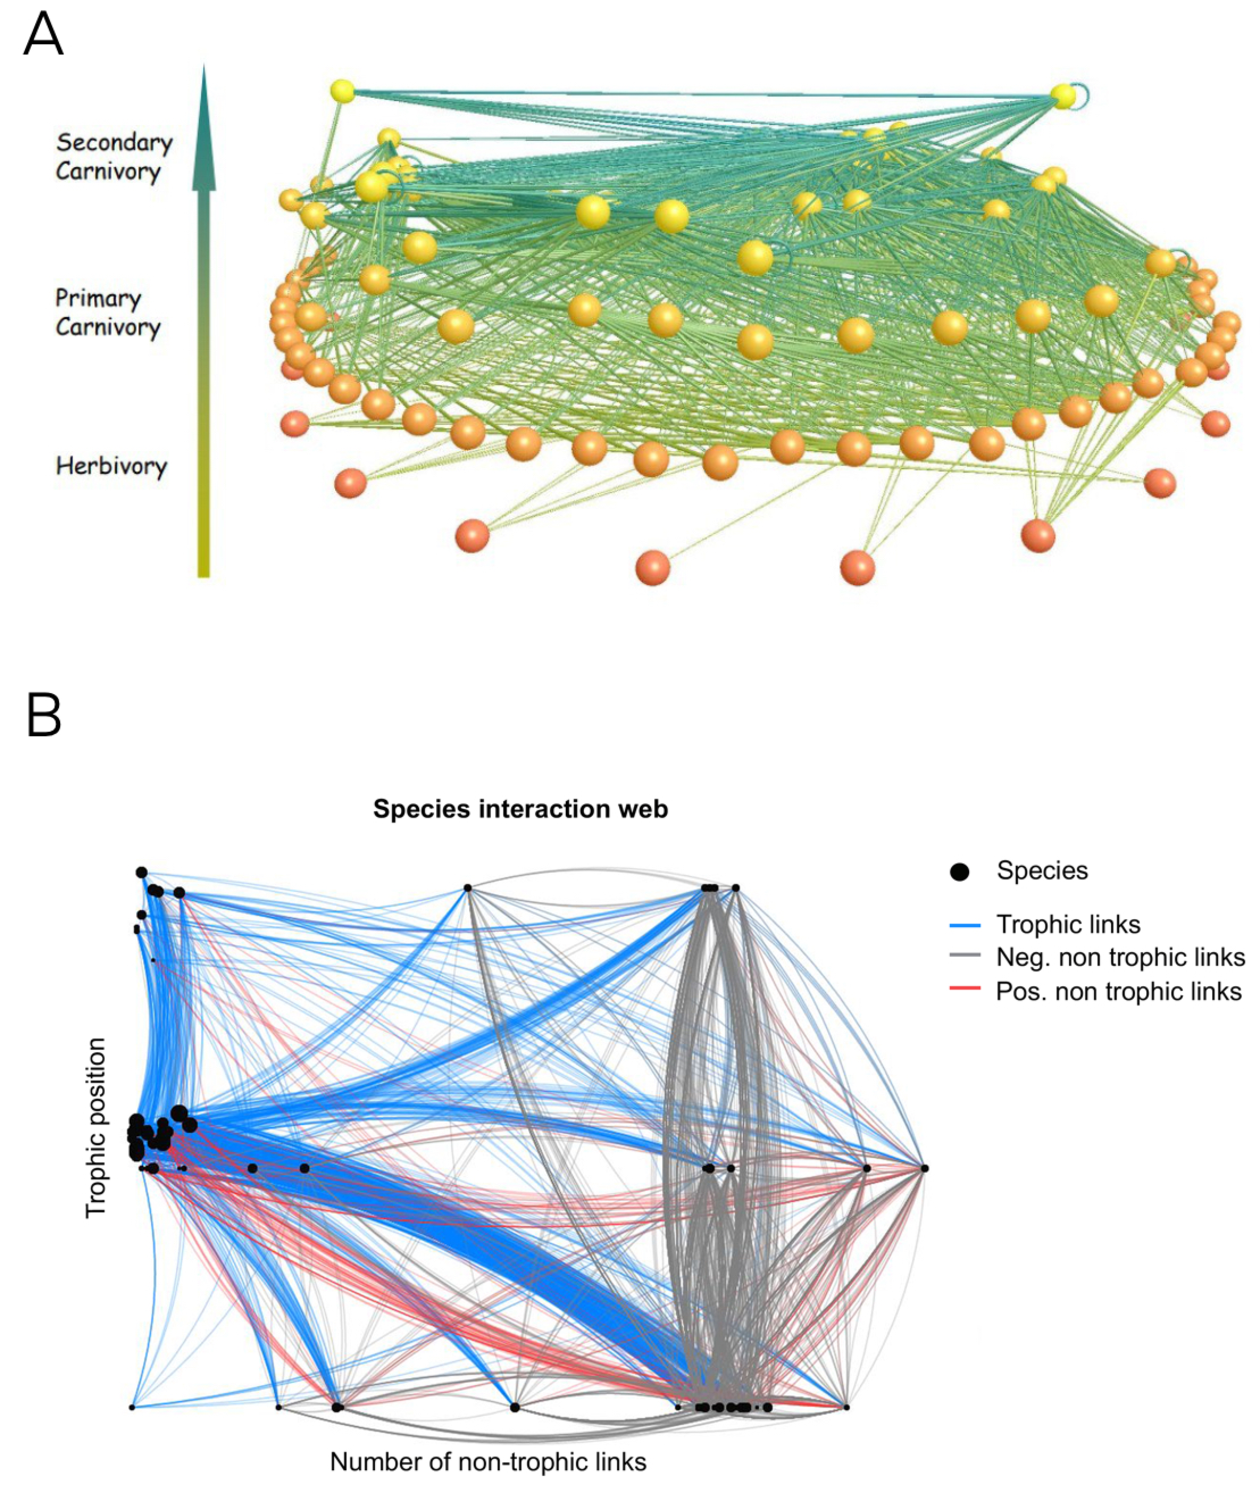
\includegraphics[width=0.8\columnwidth]{figures/methods/fig_history.pdf}
    \caption[Historical ecological networks]{(Panel a) The food Web of Little Rock Lake, Wisconsin \cite{martinez1991artifacts} was the largest food web in the primary literature for decades \cite{strogatz2001exploring}. Nodes are 181 functionally distinct \textit{trophic species} (11 fishes, 110 invertebrates, 59 autotrophs, 1 detritus). (Panel b) ``Network of trophic and non-trophic interactions between the 106 species of the Chilean web. Nodes indicate species and are sized by total degree. The vertical position is proportional to trophic level and the horizontal position is proportional to non-trophic degree. Edges are blue, red, and gray for trophic, positive, and negative interactions, respectively.'' \cite{kefi2016structured}}
    \label{chp:methods:fig:history}
\end{figure}

The sheer diversity of relations between species calls for a refinement of what interactions, and consequently links, are. More in general, one can think of two different pieces of information that can be called an interaction \cite{verhoef2010community}. First, an interaction may be a process, like the energy transfer from the resources to the consumers in food webs. In this case, they symbolize the interchange of something quantifiable like energy, nutrients, or biomass. And second, interactions may represent the \textit{effect} of a species on another. For example, if the growth of two species is enhanced when they coexist together, we deal with a positive-positive interaction. This type of interaction is called mutualism and can be generated by various processes. We have already mentioned pollination, which is a mechanism that gives rise to mutualistic interactions (Figure~\ref{chp:methods:fig:mut-comp}a). Another example is association resistance, in which a species obtains protection when it spatially associates with another species \cite{Dieckmann2000}. These mutualistic networks are described as undirected bipartite networks, sometimes weighed by the number of recorded visits for pollination or the number of co-occurrences for spatial association. The opposite effect is a negative-negative interaction, also termed competition. It can originate from trophic mechanisms, such as two predators sharing the same prey, as well as non-trophic mechanisms, like exploitative competition, when one species indirectly reduces another by  directly reducing shared resources \cite{wootton1994nature} (Figure~\ref{chp:methods:fig:mut-comp}b). \\
\begin{figure}[t]
     \centering
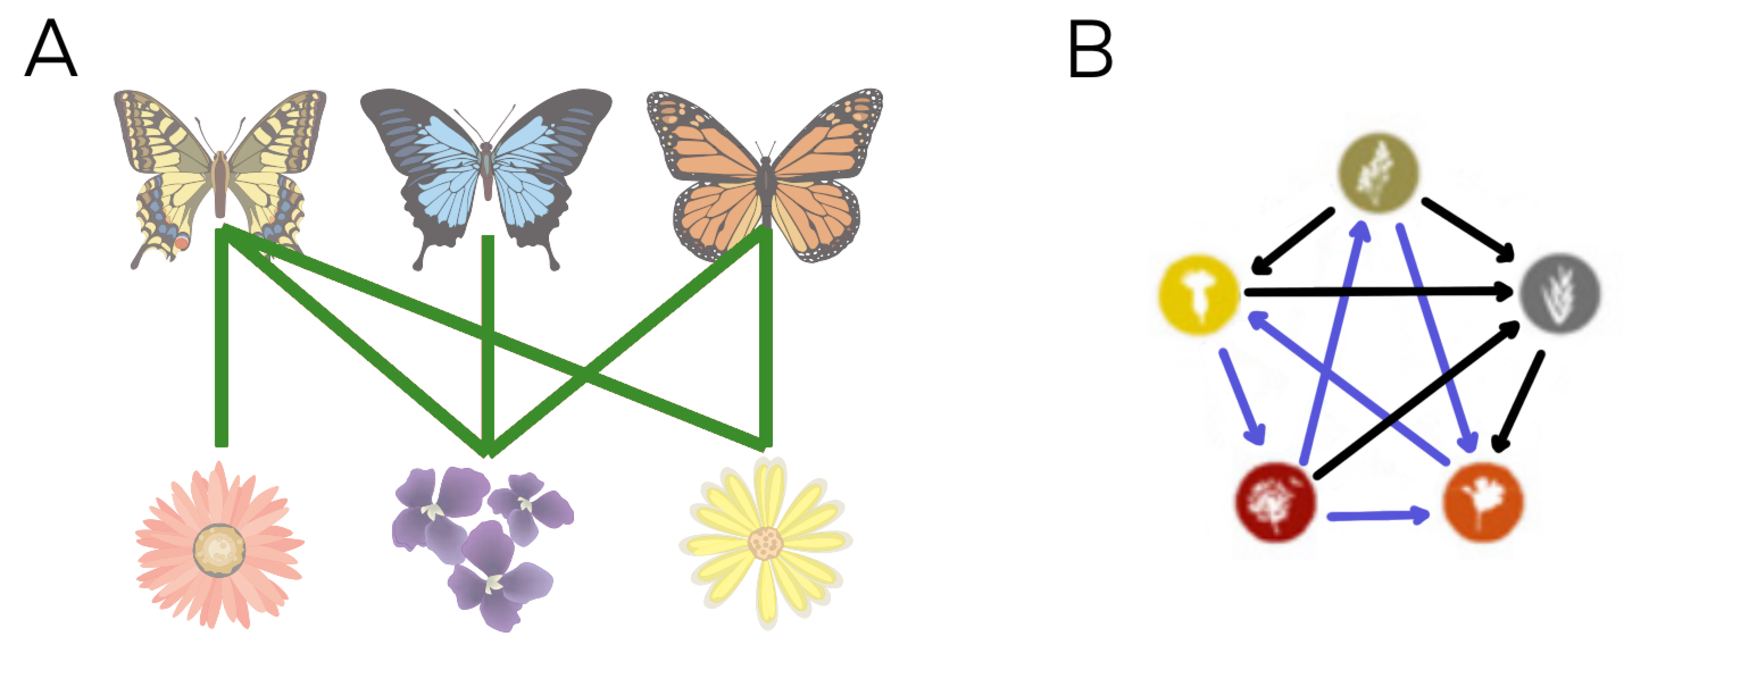
\includegraphics[width=\columnwidth]{figures/methods/fig_mut-comp.pdf}
 \caption[Mutualistic and competitive networks]{Two types of non-trophic interaction networks. (Panel a) Plant-pollinator mutualistic network. Note the bipartite division. Image extracted from \cite{rohr2014structural}. (Panel b) Competitive network. Directed links point from dominant species. Two intransitive cycles are shown in purple. Image adapted from \cite{soliveres2015intransitive}.}
\label{chp:methods:fig:mut-comp}
\end{figure}

Moreover, if several types of interactions are studied within the same representation, one can use signed networks (Figure~\ref{chp:methods:fig:history}b), or more complex structures, like multilayer networks \cite{pilosof2017multilayer} or hypergraphs \cite{golubski2016ecological}. \\

\subsection{Spatial networks}
Another type of ecological network revolves around space. In this case, nodes symbolize a location (a habitat, a patch) that can be inhabited by one or several individuals. Links represent the connections among the spatial locations. These connections can give rise to migrations, nutrient flows, or dispersal, and therefore networks may be directional and weighted. In Chapter~\ref{chp:1}, we will use a simple spatial network where nodes are spatial locations occupied by only one individual and links define seed dispersal pathways. \\

\begin{table}[t]
\centering
\caption{Types of ecological networks studied in this thesis}
\label{chp:methods:tab:networks}
\begin{tabularx}{1\textwidth}{ X X X X c}
\hline
\textbf{Network} & \textbf{Type}                                                                          & \textbf{Nodes}    & \textbf{Links}    & \textbf{Ch.}                              \\  
\hline
\hline
%Mutualistic      & \begin{tabular}[c]{@{}c@{}} bipartite\\ signed\\ (weighted)\end{tabular} & species           & interspecific non-trophic interactions & \ref{chp:2} \& \ref{chp:3}     \\
Spatial          & unsigned unweighted                      & spatial location & transfer of individuals (dispersal)    & \ref{chp:1}     \\
\hline
Mutualistic      &  bipartite signed (weighted) & species           & interspecific non-trophic interactions & \ref{chp:2} \& \ref{chp:3}     \\
\hline
Competitive      & signed (weighted)        & species           & interspecific non-trophic interactions & \ref{chp:2}  \& \ref{chp:3}     \\
\hline
Co-occurrence     & unsigned unweighted                        & individuals       & co-occurrence in the same location (overlap) & \ref{chp:3} \\
\hline
\end{tabularx}
\end{table}

\section{Ecological concepts}\label{chp:methods:ecointeract}
%%%%%%%%%%%%%%%%%%%%%%%%%%%%%%%%%%%%%%%%%%%%%%%%%%%%%%%%%%%%%%%%%%%%%%%%%%%%%%%%%%%%%%%%%%%%%%%%%%%%%%%%%%%%%

 Interactions are what connect species. They are then a central factor that drives community dynamics, one of the main subjects in ecological research. Along this thesis, we take the approach of studying the effects of ecological interactions by a parametric, or model-driven approach. We can describe these effects as a system of first-order, ordinary differential equations, i.e. equations containing functions of one or more independent variables (abundances $N_i$ or frequencies of species) and their first derivative with respect to time. We can write a general form of these systems as:
 \begin{equation}
     \frac{dN_i}{dt} = N_i f_i(N_1,... , N_S)
 \end{equation}


 In this Section, two theoretical frameworks broadly used in population and evolutionary dynamics are presented: the generalized Lotka-Volterra equations and the replicator equation. Then, we go one step further and explain a dynamical model --the niche model-- which incorporates a network construction algorithm. Finally, we discuss how a certain configuration of competitive strengths can modify the coexistence and stability of a community.

\subsection{Generalized Lotka-Volterra equations}\label{chp:methods:LV}

%The Lotka-Volterra equations were first proposed as a simple model of predation to explain the oscillatory behavior of certain fish catches in the Adriatic \cite{murray2002mathematical}. They have been quite helpful in raising relevant questions since they are able to be analytically tractable and present interesting dynamics. In fact, they were quickly generalized to include more realistic constraints and other types of interactions and to involve more than two species. \\

The generalized Lotka-Volterra model (GLV) is one of the simplest and most used nonlinear model for population dynamics of multiple interacting species. It is also a mathematical paradigm --in the sense that other models can be transformed into GLV form \cite{page2002unifying}. We can write a compact formulation of the model as:
\begin{equation}
    \frac{\textbf{dN}}{dt} = D(\textbf{N}(t))(\rho + A \textbf{N}(t))
\end{equation}
where $\textbf{N}(t)$ is the column vector of length $S$ (the total number of species) that contains the abundances of all species at time $t$, $\rho$ is the vector of intrinsic growth rates, $A$ denotes an $S \times S$ matrix of interaction coefficients, and $D(\textbf{N})$ is a diagonal matrix with the $N_i$ as diagonal elements. The intrinsic growth rates measure the growth (or decline if they are negative) of a species when it is in isolation. \\

With this representation, some important features of the community can be studied, like coexistence and stability. If $A$ is invertible, we can look for a feasible equilibrium, i.e. a solution of the equation $\rho + A\textbf{N} = 0$, where all species have positive abundances.  The stability of the stationary points can be studied through the eigenvalues of $A$. %However, since the number of parameters of the GLV grows with the number of species involved, if we choose their values at random, the community will probably collapse into smaller systems because of extinctions.\\

Regarding the possible types of dynamics, the Lotka-Volterra equations have been thoroughly studied for $2$ species, where fixed points, limit cycles around the equilibrium, and unbounded growth can appear depending on the signs and values of the elements in $A$ \cite{murray2002mathematical} 
 (Figure~\ref{fig:LV}a). When we study multi-species systems, more exotic behavior like chaos can appear \cite{houfbauer1998book} (Figure~\ref{fig:LV}b).\\ 

\begin{figure}[t]
    \centering    
    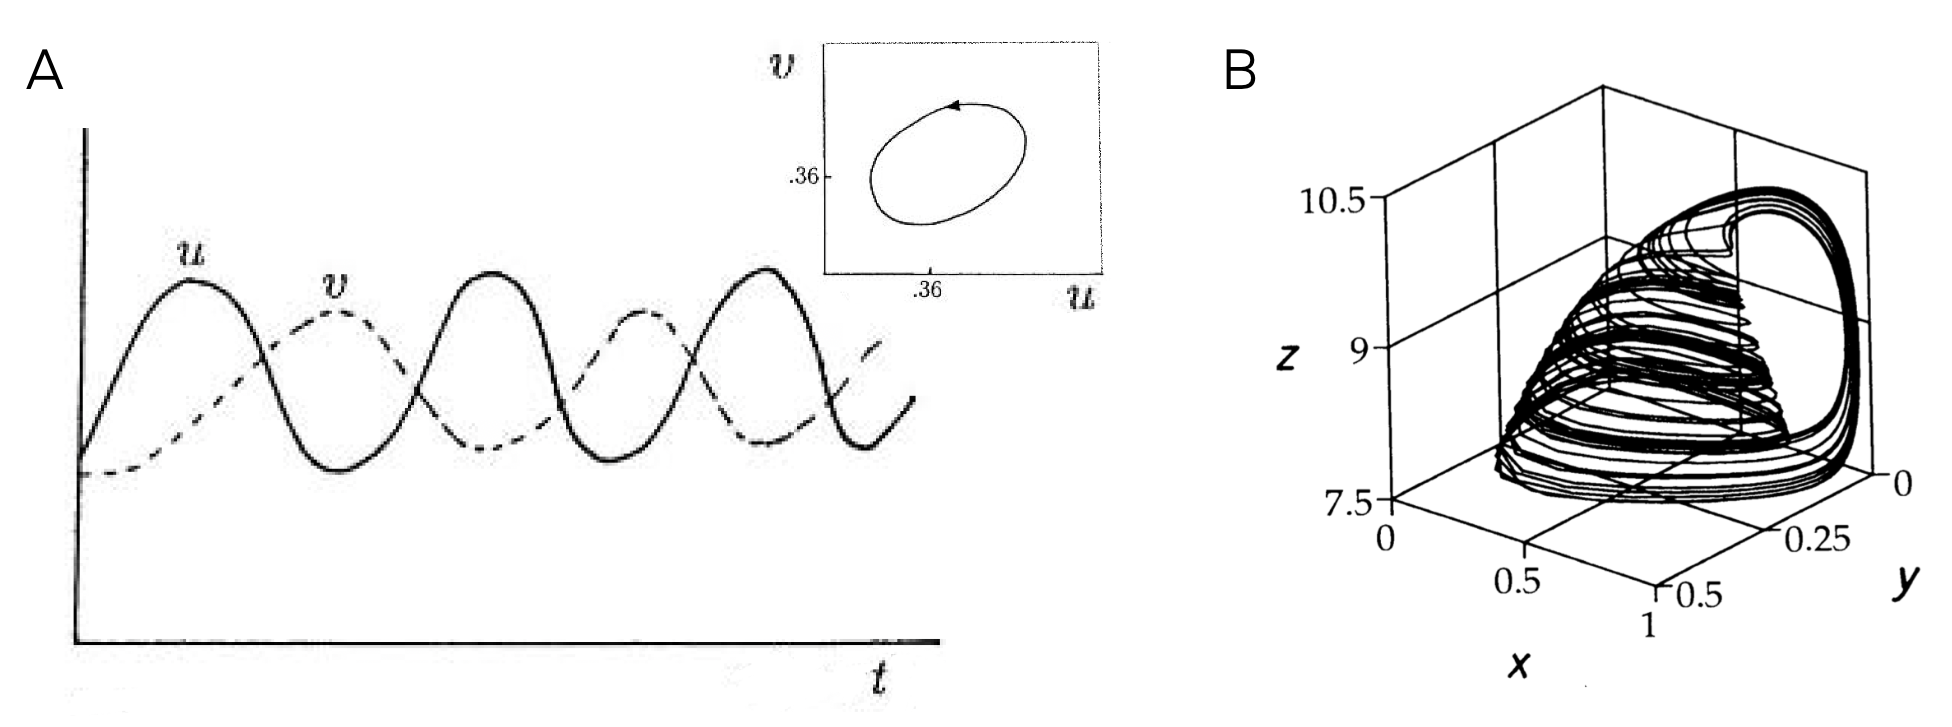
\includegraphics[width=\columnwidth]{figures/methods/fig_LV.png}
    \caption[Historical example of Lotka-Volterra equations]{The Lotka-Volterra equations were first proposed as a simple model of predation to explain the oscillatory behavior of certain fish catches in the Adriatic \cite{murray2002mathematical}. In (Panel a), we find the periodic solution for the original Lotka-Volterra equations, which only involve two species: a predator-prey system. The phase trajectory of the limit cycle is in the inset. Figure from \cite{murray2002mathematical}. These equations have been quite helpful in raising relevant questions since they can be analytically tractable and present interesting dynamics. In fact, they were quickly generalized to include more realistic constraints, other types of interactions, and to involve more than two species. For example, one can get chaos from 3 species with trophic relations. The attractor of such a system is depicted in (Panel b), from \cite{hastings1991chaos}. }
    \label{fig:LV}
\end{figure}

Within this approach, we can classify the interactions as follows: two species are in a predator-prey relationship when one population declines while the other increases, competition exists if the growth of both species decreases, and mutualism or symbiosis is the term used when both populations increase from the presence of each other. These situations are visible in the interaction matrix $A$. If, for example, two species $i$ and $j$ compete, both $A_{ij}$ and $A_{ji}$ will be negative. However, when studying different types of interactions in the same community, it is more convenient to create distinct interaction matrices for each type. Since we will study a system with mutualism and competition in Chapter~\ref{chp:3}, let's exemplify how the GLV of such a system would look by introducing a model describing the dynamics of a plant-animal community:
\begin{equation}
\label{eq:LVcm}
{\begin{aligned}{\frac {dP_i}{dt}}&=P_i \left(\rho_i^P - \sum_j \beta_{ij}^{P}P_j + \sum_k \gamma_{ik}^{P} A_k \right) \\[6pt]
{\frac {dA_k}{dt}}&=A_k \left(\rho_k^A - \sum_l \beta_{kl}^{A}A_l + \sum_i \gamma_{ki}^{A} P_i \right),
\end{aligned}}
\end{equation}
where $P_i$ and $A_k$ are the variables for the abundances of plant and animal species. The new parameters correspond to the matrices describing intra-guild competition $\beta$ and the mutualistic interactions $\gamma$. Examining the mutualistic benefit, we see that its effect gets stronger with larger species abundance. However, the effect is far from linear, as is supposed in the previous equation. A typical assumption is a mutualistic response that saturates \cite{bastolla2009mutualism,rohr2014structural, suweis2013emergence}:
\begin{equation}
\label{eq:LVcmholling}
{\begin{aligned}{\frac {dP_i}{dt}}&=P_i \left(\rho_i^P - \sum_j \beta_{ij}^{P}P_j + \frac{\sum_k \gamma_{ik}^{P}A_k }{1+ h \sum_l \gamma_{il}^{P} A_l} \right) \\[6pt]
{\frac {dA_k}{dt}}&=A_k \left(\rho_k^A - \sum_l \beta_{kl}^{A}A_l + \frac{\sum_i \gamma_{ki}^{A}P_i }{1+ h \sum_j \gamma_{kl}^{A} P_j}\right).
\end{aligned}}
\end{equation}
The fraction in these modified Lotka-Volterra equations is called Holling Type-II functional response and imposes a limit to the mutualistic effect by adding a handling time $h$. This restriction considers that species are unable to engage with a high number of mutualistic partners because each interaction involves time. With this functional response, the benefit from mutualistic interactions does not increase monotonically as the number of species increases, bounding the dynamics.
%A typical derivation of Type-II response assumes that handling a ''unit'' of consumer prey takes Th time, with Ts time spent searching and Tt total time, giving: Tt = Ts + ThY with the amount of prey caught Y .
%less prey = limitation is the finding factor.
%lots of prey = saturation = limiting is h.




%%%%%%%%%%%%%%%%%%%%%%%%%%%%%%%%%%%%%%%%%%%%%%%%%%%%%%%%%%%%%%%%%%%%%%%%%%%%%%%%%%%%%%%%%%%%%%%%%%%%%%%%%%%%%
\subsection{Replicator dynamics}\label{chp:methods:repli}
 The replicator equation is a well-known equation in evolutionary game theory \cite{houfbauer1998book}. It assumes that the strategies of the game --actions that rational players choose to play-- are selected according to their frequency $x_i$. The equation sets how the evolution of these frequencies, $\dot{x_i}$, varies according to its rate of success. We will use the replicator dynamics in Chapter~\ref{chp:2} to model species frequencies instead of strategies, so we will continue the description of the dynamics with $n$ species in mind rather than strategies. \\
 
The replicator equation captures the intuitive idea that species that do well grow faster. To quantify how well a species is doing, the local fitness of a species, $f_i$, is used. Fitness is a broad concept with several definitions depending on the context. Here, it is just a linear combination of the species frequencies given by payoffs $a_{ij}$ that account for the reproductive success:
\begin{equation}
    f_i = \sum_{j = 1}^{n}  a_{ij} x_j.
\end{equation}\label{eq:localfitness}
 Thus, the replicator equation is a phenomenological description of the system. It only tells us that the fitness of species $i$ will increase by $a_{ij} x_j$ if the interaction occurs, but it does not take into account how species $i$ and $j$ interact. \\
 
 More precisely, $x_i$ varies according to the difference between its local fitness and the average fitness of the population,  $ \phi = \sum_{j} x_j f_j = \sum_{j,k} x_j a_{jk} x_k$, and the evolution equation reads
 \begin{equation}
    \dot{x_i} = x_i \left( \sum_j a_{ij} x_j - \sum_{j,k} x_j a_{jk} x_k \right),
    \label{chp:methods:eq:replicator}
\end{equation}
 where $(a_{ij})$ is the so-called payoff matrix. Species $i$ will grow if the first term inside the parentheses is greater than the average fitness of the community of $n$ species. In this context, we can interpret fitness as how well a species will grow according to its interactions. \\
 
 Regarding the possible solutions, they are all confined in the $(n-1)$-simplex, the set of non-negative points $(x_1, ..., x_n)$ whose coordinates are all non-negative and add up to one. This is simply a consequence
 of working with the frequencies of the species, which have the property $\sum^n_{i = 1} x_i = 1$.
For the case of two species, at most one isolated equilibrium where $x_i > 0, \, \forall i$ (i.e. in which no species going extinct) can be reached \cite{Nowak2006EvolutionaryDynamics}. As the number of species increases, more exotic behavior can occur. For example, if $n \geq 4$, the possibility of chaos appears. Moreover, the replicator equation is mathematically equivalent to the Lotka-Volterra equations \cite[Chapter~7]{houfbauer1998book}, so whatever outcome is true for one equation will hold for the other\cite{page2002unifying}.\\
 
During this thesis, we will consider the replicator dynamics on a graph, where each node is occupied by a different species. The payoff matrix elements $a_{ij}$ are now zero if species $i$ does not interact with species $j$, and  equals an interaction strength value $\alpha_s$  otherwise. The diagonal terms are fixed to $c < 0$, since the effect a species has on itself is usually regulatory. In the extreme case where none of the species interact with each other ($a_{ij} = 0 \forall i,j$), the local fitness equals the average fitness, and the system remains in its initial condition. In the all-to-all case (when every species interacts with every other species), the $n$ species coexist with density $x_i = 1/n$. Other configurations yield different solutions, usually involving the extinction of several species. Their full analysis will be carried out in Chapter~\ref{chp:2}.
%%%%%%%%%%%%%%%%%%%%%%%%%%%%%%%%%%%%%%%%%%%%%%%%%%%%%%%%%%%%%%%%%%%%%%%%%%%%%%%%%%%%%%%%%%%%%%%%%%%%%%%%%%%%%%%%%%%%%%%%%%%%%%%%%%%%%%%%%%%%%%%%%%%%
\subsection{Niche theory and beyond}\label{chp:methods:niche}
Since the presence of ecological (and evolutionary) processes is encoded in the network, we ask about the mechanisms that give rise to the observed network structure. Some basic models may produce communities with realistic topologies. One such approach is the niche model \cite{cai2021niches}. Its main idea is that species choose their interaction partners to maximize their abundance.\\

The niche model incorporates the elusive concept of niche, and adaptive species connection dynamics. The niche is interpreted here in line with Hutchinson's fundamental niche: the hypervolume defined by the limiting factors of the species growth \cite{hutchinson1957concluding}. These include the environmental conditions that allow species to satisfy their minimum requirements, so that the death rate of a local population is equal to or smaller than the birth rate \cite{chase2009niches}. \\

The idea of using niches to infer network structure was initially developed for food webs \cite{williams2000niche}, and it has been recently adapted to mutualistic communities \cite{cai2021niches}. We will introduce the model in this latter context, through a pollinating community with two guilds: plant species $P$ and pollinators $A$, where there is competition inside guilds and mutualism across guilds. \\

The key aspect of the model is that every species is randomly assigned a \textit{niche profile}, which is a region on the abstract one-dimensional niche axis $s$. The niche axis represents the operating or living range of the species and is shared by all species within a guild. The region can be defined in several ways, like an interval (typically in food webs), or a Gaussian function. We will continue the presentation of the model with a Gaussian function for illustrative purposes, but in Chapter~\ref{chp:3} cosine similarity will be used.  Hence the niche profile is a statistical distribution of the resources used by a given species. We define \textit{niche overlap} as the overlapping between niche profiles of two species. For within-guild overlaps, is given by:
\begin{equation}
    G^{PP}_{i j}  =  \int G_i^P(s) G_j^P(s) ds,
\end{equation}
 where $ G_i^P(s)$ is the Gaussian profile of plant species $i$. The overlap quantifies the niche similarity of species and is a proxy for competition within the guild. Species with highly overlapping niches are thought to compete for the same set of limited resources, for example, resources related to habitat conditions like soil pH or similar nesting sites. For cross-guild overlaps, we get:
\begin{equation}
    G^{PA}_{ik}  =  \int G_i^P(s) G_k^A(s) ds.
\end{equation}
In this context, the overlap captures the niche complementarity of mutualistic partners. This is based on the assumption that both partners must live in the same environment for the mutualistic relationship to occur. For example, pollinators must be fully developed when the flower is functional, i.e. close physical proximity between the organisms is required.\\

Then, it is assumed that species abundances evolve following some dynamics and, as mentioned earlier, that species can adapt their connections. In our version of the model developed in \cite{palazzi2021ecological}, the driver behind the adaptation is the maximization of abundance.  Niche overlap comes into play here because it is coupled with the strength of the interactions. Higher overlap leads to more intense interactions. The model develops as follows: a randomly selected species tries to connect to a different mutualistic partner, removing one of its previous links. If the abundance of the species rises, the rewiring is accepted; otherwise, it is rejected (Figure~\ref{fig:nicheModel}b).  To reflect the fact that it is harder to remove links from a specialist than from a generalist species, the rewiring probability of a species is proportional to $p_{PA} \propto 1 - k_{P}^{-1}$. Between rewiring attempts, we wait until the population dynamics has reached an equilibrium. \\

The number of species and the connectance of the networks of interactions (which are conserved through the optimization process) can be empirical values. In this way, the model can reproduce key patterns in food webs as the fractions of species at the top, intermediate, and basal
trophic levels \cite{williams2000niche}, or to explain the emergence of patterns of nestedness and in-block nestedness \cite{suweis2013emergence,cai2021niches} in mutualistic networks (Figure~\ref{fig:nicheModel}a). In Chapter~\ref{chp:3}, we will apply the model to a non-biological system, the user-hashtag partnerships, because mutual benefits exist in this context too.
 \begin{figure}[t]
 \centering
   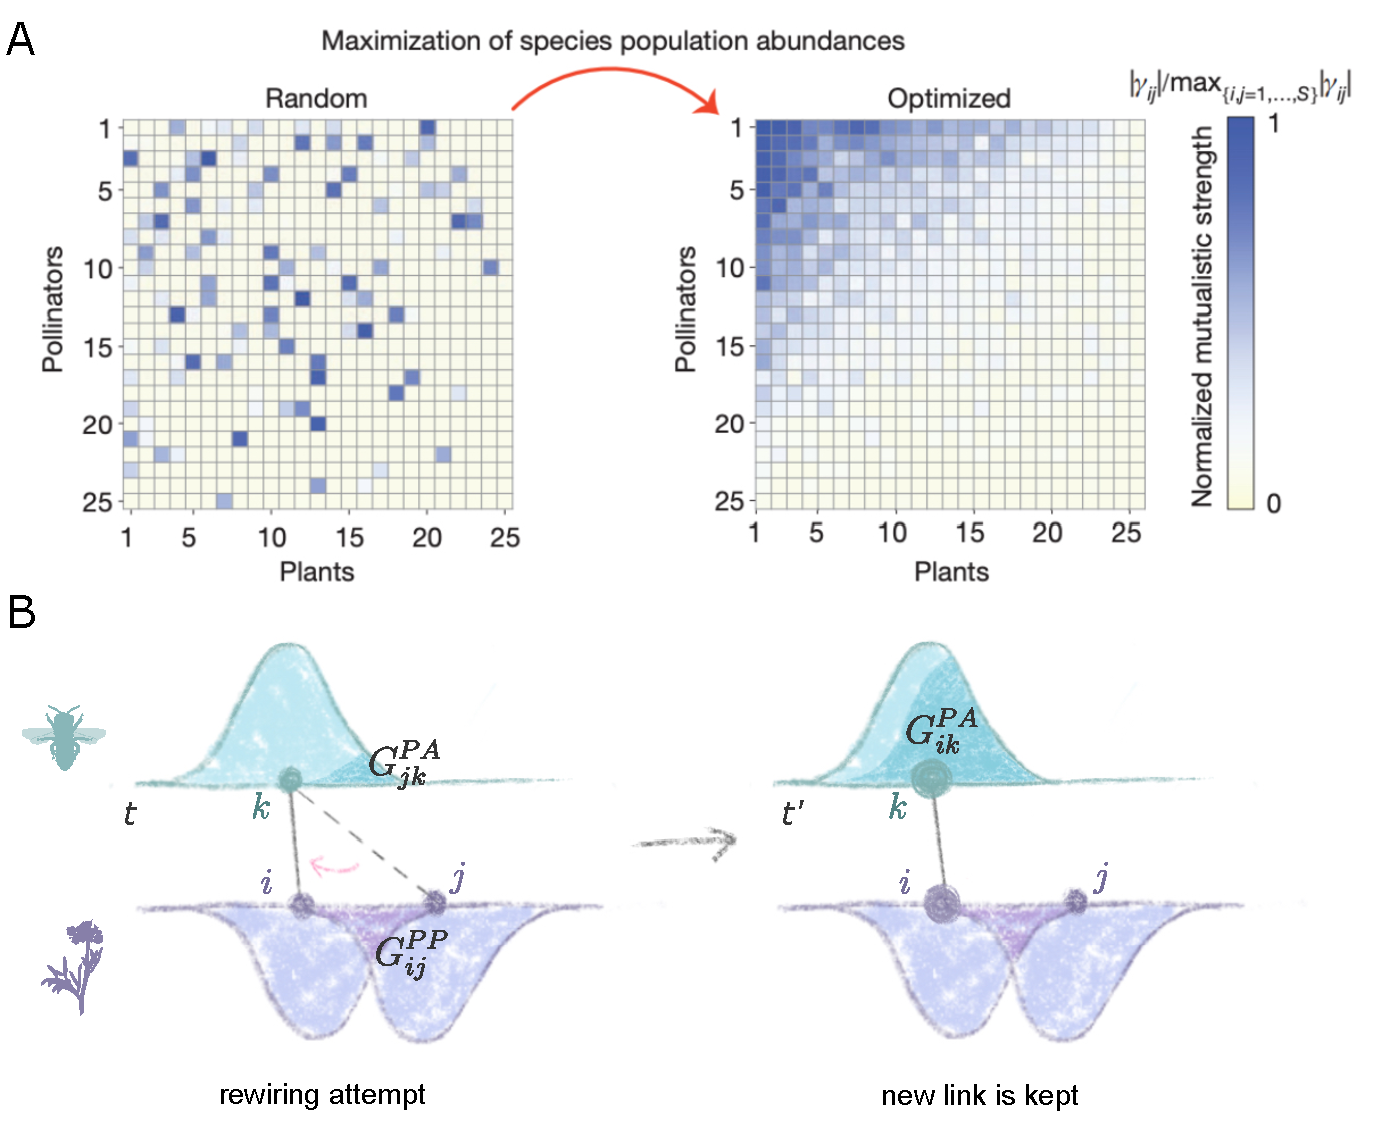
\includegraphics[width=\columnwidth]{figures/methods/niche.pdf}
    \caption[ Schematic representation of the niche model]{(Panel a) Abundance optimization leads to nested networks in ecological communities. Figure from \cite{suweis2013emergence}. (Panel b) Schematic representation of the niche overlaps and rewiring. In the example, node size symbolizes abundance and darker areas are niche overlaps. A pollinator $k$ rewires to a new partner flower $i$ with higher niche overlap ($G^{PA}_{ik} > G^{PA}_{jk}$). Since the abundance of the pollinator rises, the new link (solid line) is accepted. Images of pollinator and plant are available under CC0 $1.0$  license.}
   \label{fig:nicheModel}
\end{figure}
%Images of pollinator $Megachile\, Rotundata$ and plant $Crithmum\, maritimum$ available under CC0 $1.0$  license.
%%%%%%%%%%%%%%%%%%%%%%%%%%%%%%%%%%%%%%%%%%%%%%%%%%%%%%%%%%%%%%%%%%%%%%%%%%%%%%%%%%%%%%%%%%%%%%%%%%%%%%%%%%%%%%%%%%%%%%%%%%%%%%%
\subsection{Intransitivity}\label{chp:methods:intra}
\epigraph{… by chasing your victim faster, you actually help out the guy who’s chasing you.}{\textit{Kerr et al.} \cite{kerr2002local}}
Competition plays a vital role in the evolution and maintenance of ecosystems. In fact, one of the long-standing questions in ecology is why there are so many species despite competition. A possible solution that has been proposed is making competition --a negative interaction often related to struggle and hassle-- work for biodiversity. But not all sorts of competition are useful to promote coexistence. In particular, researchers have considered a concrete arrangement of competitive interactions that is not hierarchical: intransitive interactions \cite{soliveres2018everything}. \\

When a community presents a hierarchical competitive structure, species could be sorted according to how well they outcompete each other. When competing for the same set of resources and with no other mechanisms at play, we would eventually find that the species with the highest ranking would have total predominance. All the others would become extinct since they perform worse. This situation is called the principle of competitive exclusion. On the other hand, with non-hierarchical interactions, if species $A$ outcompetes species $B$ and $B$ outcompetes species $C$, then species $C$ outcompetes species $A$. In such circumstances, there are no clear weak species. The abundance of the different species will cycle \cite{may1975nonlinear}, preventing one single species from taking over the whole population.  A well-known example of such cycles is the rock-paper-scissors game (Figure~\ref{chp:methods:fig:RPS}).  \\

\begin{figure}[t]
     \centering
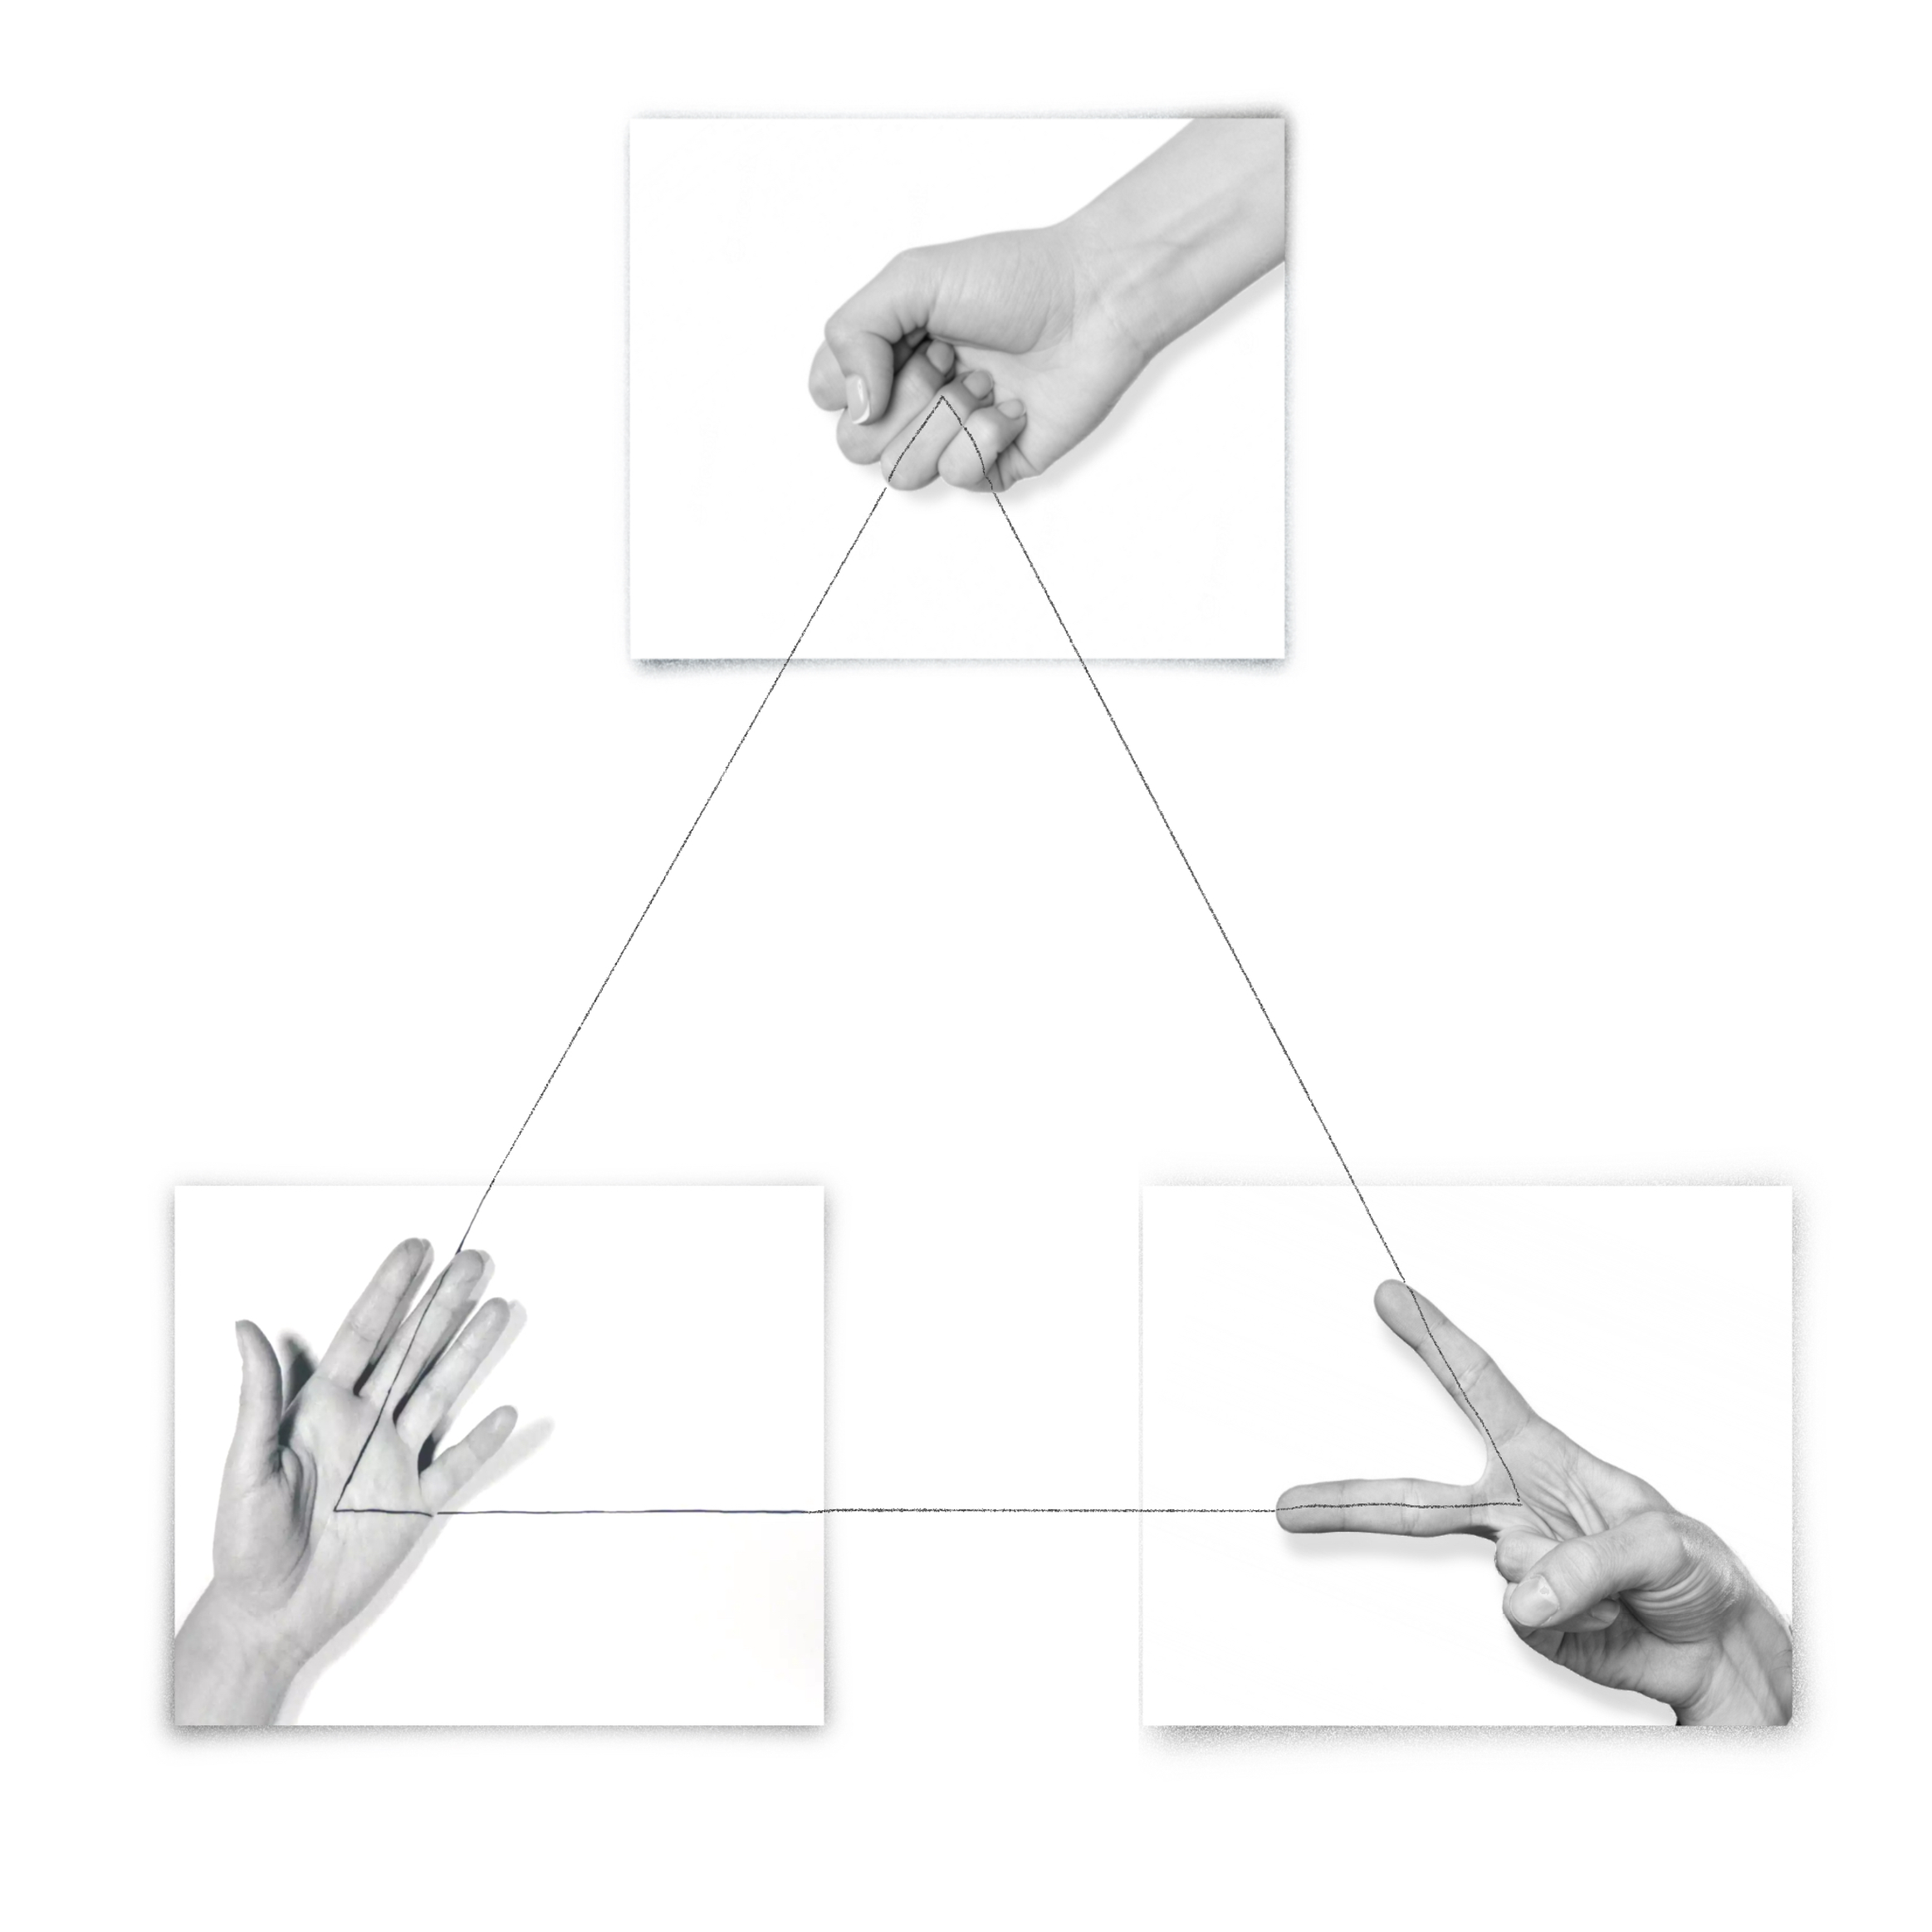
\includegraphics[width=0.7\columnwidth]{figures/methods/fig_RPS.pdf}
 \caption[Intransitivity diagram]{In the common playground game, rock crushes scissors, scissors cuts paper, and paper covers rock. No strategy has an advantage, there is no hierarchy, and because of this, multiple species may coexist by cycling in and out of dominance. Image inspired on Liliana Porter's wall installation ``Untitled (triangle)'' (1973).}
\label{chp:methods:fig:RPS}
\end{figure}

 There are some classic examples of intransitivity in natural systems, such as the side-blotched lizards \cite{sinervo1996rock}. The male lizards use, depending on their throat color, three different mating strategies that form an intransitive cycle, creating oscillations in color dominance over the years. Another seminal work is the one conducted on \textit{E. coli} by Kerr \textit{et al.} \cite{kerr2002local}, where three strains regulate the resistance, sensitivity, and production of a toxin. In theory, they form an intransitive cycle, but coexistence only actually occurs if their movement is constrained in a Petri dish. However, these behaviors, which can easily arise in simple mathematical models of $3$ or more species \cite{may1975nonlinear}, have proven in general to be difficult to find in nature \cite{godoy2017intransitivity, friedman2017community}.\\

%Despite these works suggesting that intransitivity is hard to find, a species cannot be great at everything. This opens a door to intransitive effects, and all that remains is where to find them. 
A possibility is to abandon small communities --3 lizards, 3 bacteria-- and study systems with a larger number of organisms. The reason lies in the simple, but not for that less powerful idea that biodiversity begets biodiversity \cite{maynard2017diversity}. If the number of species in a community is high, it is likely that they had very different competitive strategies and evolutionary histories. More species open the possibility of more potential and realized interactions. In this case, intransitive interactions can form, creating a self-reinforcing protection against competitive exclusion. Furthermore, recent studies have paired intransitive interactions with auxiliary mechanisms, such as spatial constraints \cite{Laird2015} or mobility \cite{reichenbach2007mobility}, to obtain stable systems. In Chapter~\ref{chp:1}, we will investigate how the locality of interactions affects the dynamics of intransitive communities.\\

%In fact, plant communities are species-rich assemblages where intransitive interactions have been empirically found. Intransitive competition occurred in more than $65\%$ of the sites in a study involving drylands and agricultural grasslands \cite{soliveres2015intransitive} and was associated with higher biodiversity. However, another empirical work found that intransitivity was uncommon in annual plant communities \cite{godoy2017intransitivity}. \\

%The dearth  (for now) of empirical data has not stopped researchers from developing more advanced computational models. Their main characteristic is that intransitivity is paired with auxiliary mechanisms not only to violate the principle of competitive exclusion, but also to get rid of oscillations and obtain a stable system. After all, oscillations in discrete systems may end up in extinctions if they are wide enough \cite{may1975nonlinear}. In another theoretical work, intransitive cycles are combined with mobility, obtaining a critical threshold below which mobility sustains species diversity \cite{reichenbach2007mobility}.
%According to the works in these lines,  a number of requirements should be met in order for intransitive communities to emerge and persist \cite{permogorskiy2015competitive}. As a summary:
%\begin{enumerate}
%    \item The system has a potential appropriate diversity. Too small systems stagnate and die out by cascades of extinctions.
%    \item The interactions take place in a relatively limited stable space. External disturbances are minimal.
%    \item The development of competitive abilities carries a cost. There are trade-offs.
%\end{enumerate}
%HOI or mobility are just some examples of intransitivity's companions that emphasize the importance of taking other factors into account when disentangling the bank. 

%Summing up, theoretical models suggest that intransitive competition plays a significant role in promoting species coexistence, although there is currently insufficient empirical data to draw any firm conclusions. In fact, whether intransitivity is common or rare in nature and its importance in real ecosystems is still an open question.
%%%%%%%%%%%%%%%%%%%%%%%%%%%%%%%%%%%%%%%%%%%%%%%%%%%%%%%%%%%%%%%%%%%%%%%%%%%%%%%%%%%%%%%%%%%%%%%%%%%%%%%%%%%%%
\subsection{Macroecological patterns}\label{chp:methods:macro}
Observing nature as Darwin and Wallace did is just the first step to truly understanding its complexity. As a next step, ecologists have traditionally had a hypothetico-deductive, often experimental approach, where a small and defined part of an ecosystem was taken apart to study how it works. This reductionism, whose success should not be discounted, has a particularly important limitation in ecology:  the results of microscopic studies cannot easily be extrapolated to larger scales, hindering a complete synthesis of the understanding of the structure and dynamics of ecosystems. A lot of replications should be made in different habitats and latitudes, and there are simply not enough resources to carry them, making it difficult to place results in a broader perspective. \\

A complementary step is to keep track of what is observed to analyze the patterns and behaviors that emerge. This is the essence of macroecology, an approach that focuses on patterns and relationships at large spatial and temporal scales \cite{brown1995macroecology}. It emphasizes the study of biodiversity and ecological processes across different geographic regions. The goal of macroecology is to identify and understand the broad-scale ecological patterns –macropatterns– and processes that shape the distribution and abundance of species and ecosystems. Certain universal rules have been discovered \cite{verberk2011explaining}, such as the fact that larger habitats tend to have more species than smaller ones. Additionally, it is almost always the case that in any community of species, there are a few species that are very abundant and many more that are rare. \\

One of the key patterns in macroecology is the species-area curve, which describes the relationship between the size of a geographic area and the number of species that can be found within it. This relationship is often depicted by plotting the number of species observed in a sampled area against the size of that area. The species-area curve typically follows truncated scale-free behavior, which means that the number of species increases rapidly with the area at first, but then levels off as the area becomes very large. \\

Macroecological research not only offers greater potential for generality but also presents a powerful tool for prediction. Patterns have been used from estimating the total number of species on Earth \cite{mora2011many} to predict how many species are likely to be lost as a result of habitat destruction and other human activities. For example, faced with this latter problem, researchers in exploit data on the species-area curve of the fauna of isolated mountain ranges to predict the species that would go extinct under climate warming, without detailed knowledge of their population biology \cite{mcdonald1992using} (Figure~\ref{chp:methods:fig:exmacro}).\\

\begin{figure}[t]
     \centering
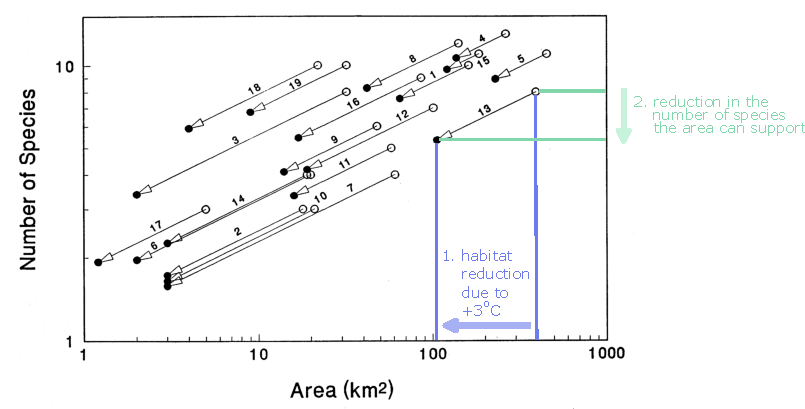
\includegraphics[width=\columnwidth]{figures/methods/fig_ex_macro.pdf}
 \caption[The macroecological approach]{The species-area curve for the distribution of mammal species among isolated mountain ranges. The researchers first used available information to obtain how much habitat loss would cause an assumed $3^{\circ}$C warming.
The arrows represent the changes in both area and number of species resulting from climatic change: the  open circles indicate the current number of species, and the solid circles indicate the predicted number that will persist following a temperature increase. Numbers identify the mountain ranges. Figure adapted from \cite{brown1995macroecology}.}
\label{chp:methods:fig:exmacro}
\end{figure}

Overall, macroecological approaches have led to a paradigm shift because they seek to understand ecological systems through global statistics instead of particular models for each community. Carrying a comprehensive analysis allow researchers to reveal features previously unknown. And this can pave the way for the creation of models and policies.

%%%%%%%%%%%%%%%%%%%%%%%%%%%%%%%%%%%%%%%%%%%%%%%%%%%%%%%%%%%%%%%%%%%%%%%%%%%%%%%%%%%%%%%%%%%%%%%%%%%%%%%%%%%%%
\section{Computational social science}\label{chp:methods:CSS}

\epigraph{A field is emerging that leverages the capacity to collect and analyze data at a scale that may reveal patterns of individual and group behaviors.}{\textit{Lazer et al.} \cite{lazer2009computational}}
Technology has profoundly changed our lives. It is crucial to understand the structure and nature of these changes to face new social challenges such as the  unethical use of communication systems, together with social, economic, and political division. Specially disrupting have been the changes in our communication channels, which can give rise to the spread of fake news, exposition of sensitive and private data, and other cyber risks.\\

The introduction of information and computation technologies (ICT) has also come with new tools to tackle the challenges it has generated.  ICT generate data, \textit{big} data, which can provide insight into the processes at the societal level. We can take advantage of this massive amount of data to create predictive and explanatory models of society. This new approach to the study of society has been called Computational Social Science \cite{lazer2009computational,lazer2020computational}. \\

Computational social science is an interdisciplinary discipline that combines social science research with complexity  and computer science to provide new insights into human behavior and society. The fact that computational social science involves several other disciplines is rooted in the nature of social systems themselves. Essentially, social systems are inherently complex, since they present emergent phenomena, and interdependencies
and feedback across the micro and macro levels of organization \cite{conte2012manifesto}.\\

\begin{figure}[t]
     \centering
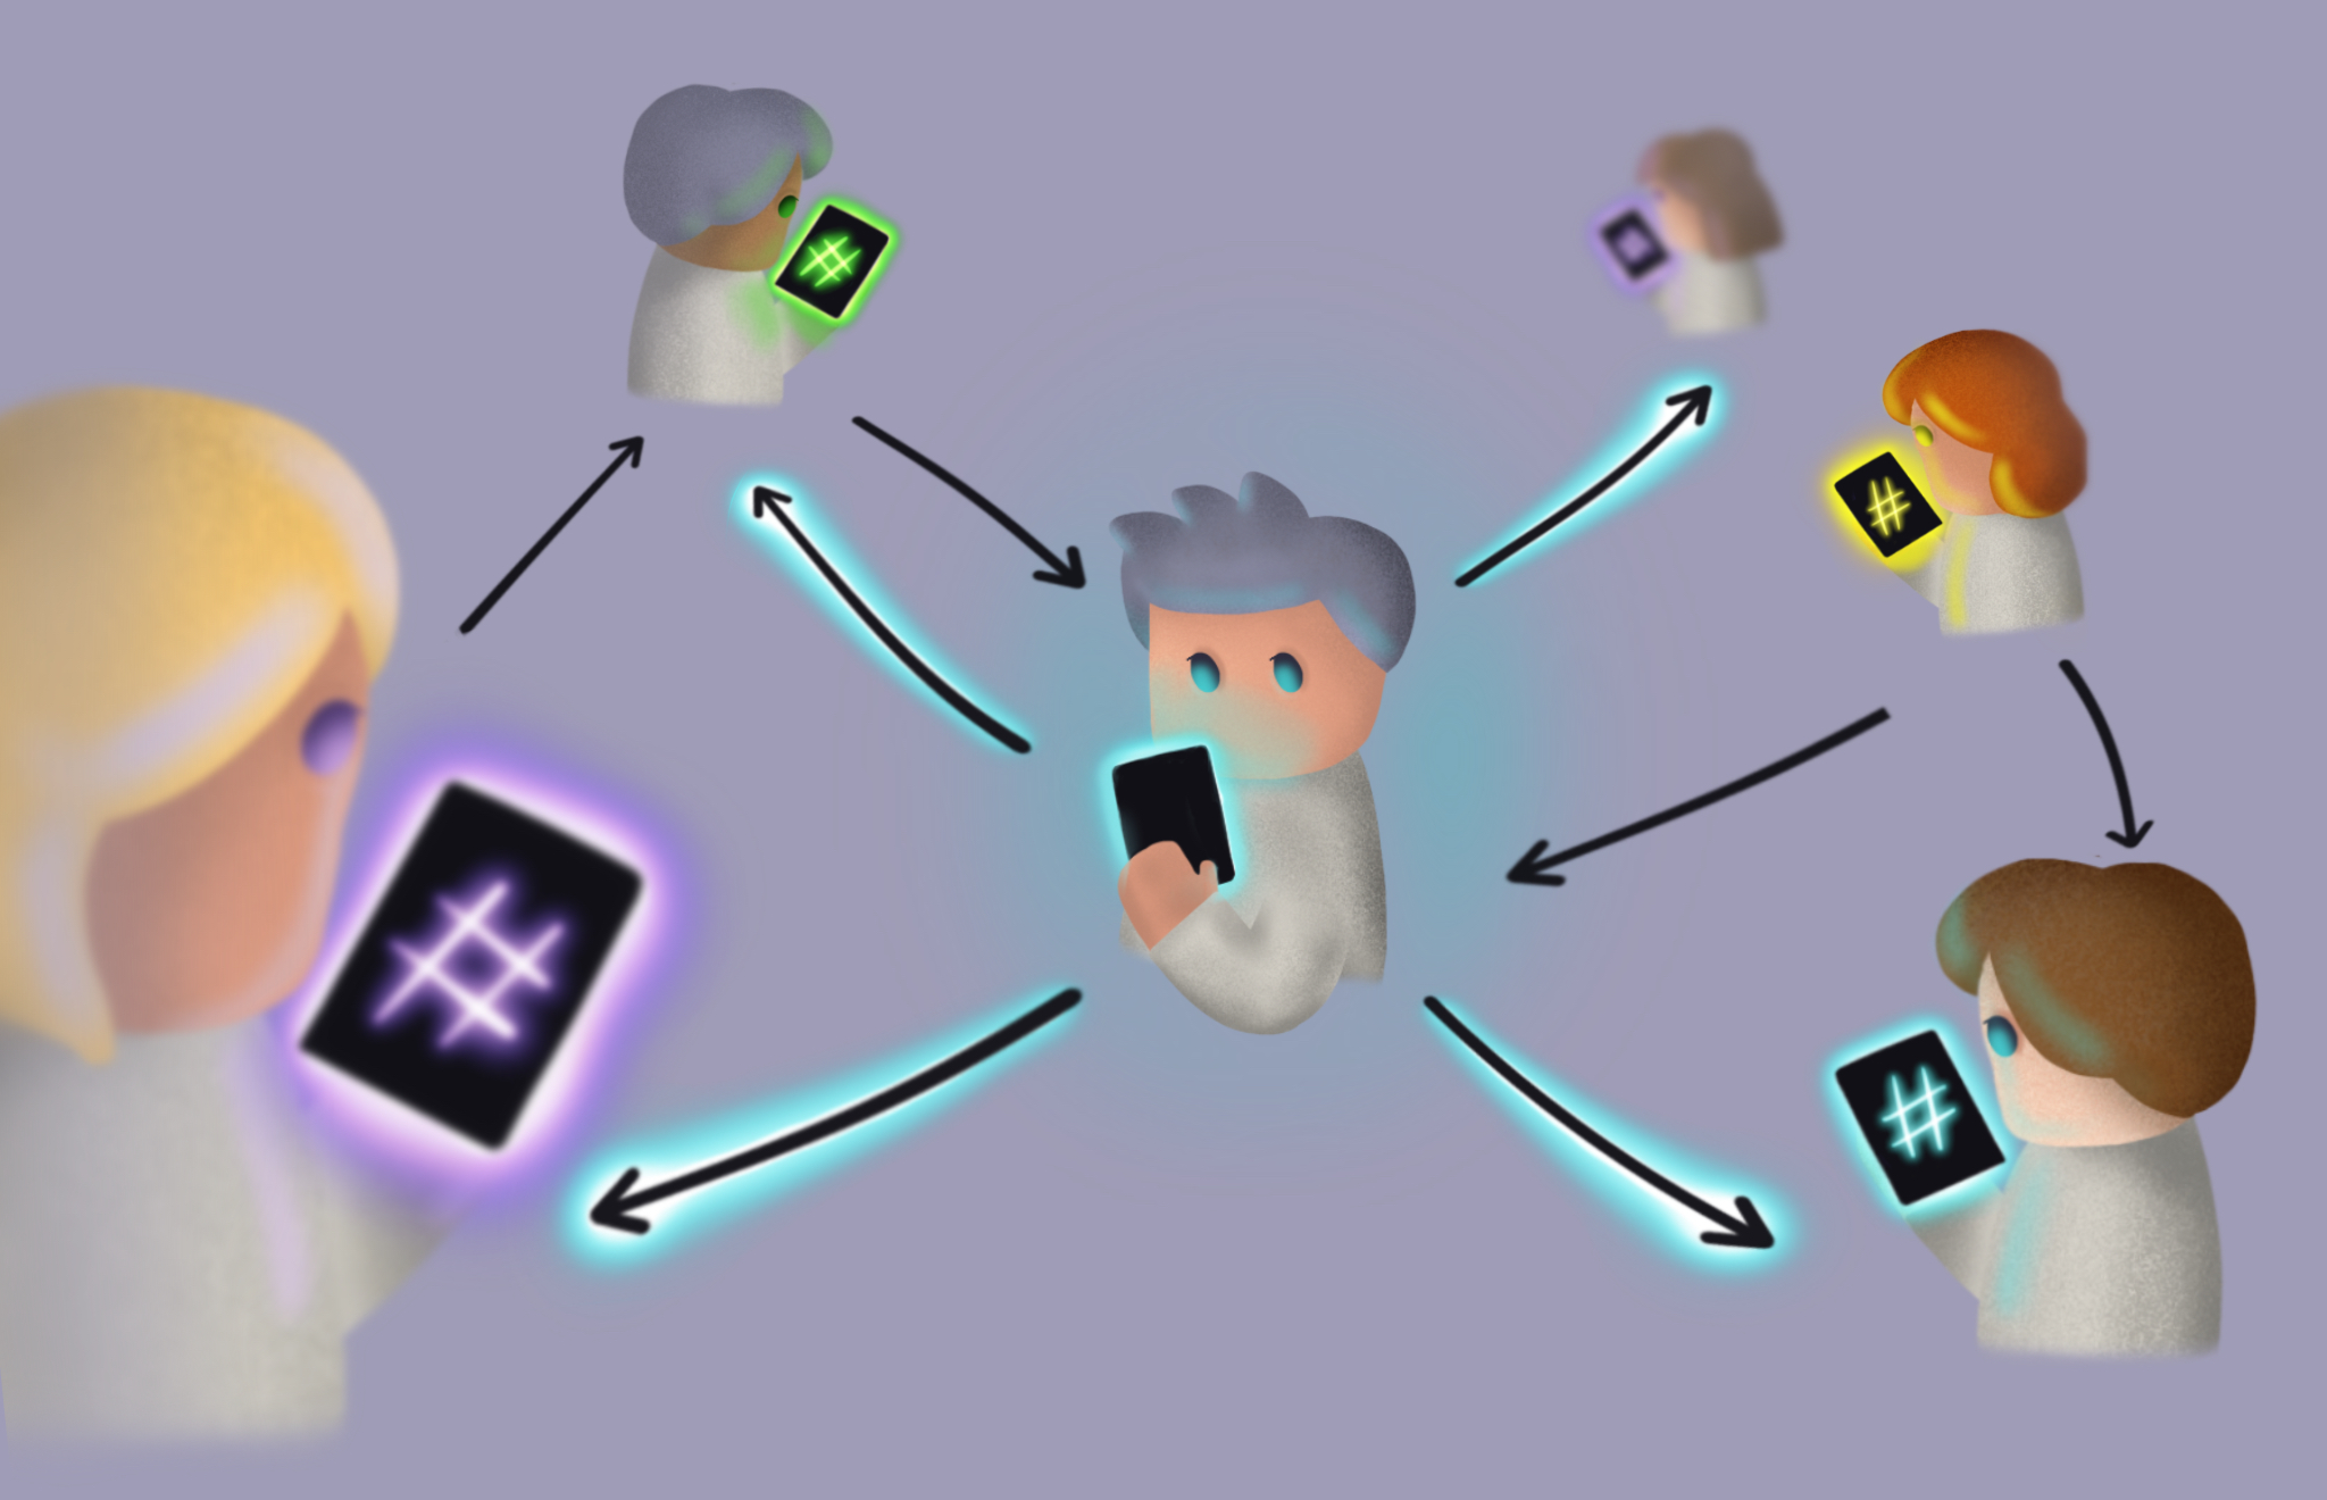
\includegraphics[width=0.8\columnwidth]{figures/methods/fig_neutral.pdf}
 \caption[Online social network dynamics]{Online social networks have been recently studied in computational social science. They are virtual structures made of individuals using the Internet as a communication medium for interacting and sharing content and opinions. Online social networks allow millions 
users worldwide to produce and consume content, providing
access to a vast source of information on an unprecedented
scale. It has become increasingly evident that
competition significantly shapes the structure and the dynamics of these information-driven platforms: users thrive
for visibility, while memes can be thought of as entities that
compete for users’ attention. Each user in the network pays
attention to a finite number of memes constrained by her finite capacity.}
\label{chp:methods:fig:neutral}
\end{figure}

Computational social science uses data from ICT to create quantitative, qualitative, and virtual models, which revolve around some aspects of social systems. For instance, nowadays communication is fast to produce and cheap to consume. This new situation has accelerated the diffusion and contagion of cultural traits in social media. To explain the empirical data that supports the acceleration, mathematical models based on competition for finite collective attention have been proposed \cite{palazzi2021ecological,lorenz2019accelerating}. These models allow us to understand the ups and downs of popular
content and the changes in the online network structure (Figure~\ref{chp:methods:fig:neutral}). \\

The characterization of the propagation of information in social media is another challenge that computational social science is addressing.  It has been discovered that this propagation generates identical macroscopic patterns across different platforms. In turn, the existence of the patterns has helped to discover, using statistical tools borrowed from physics, that bursts of activity in online communication systems can be described by complex contagion dynamics \cite{notarmuzi2022universality}.\\

In this thesis, we address two current challenges of computational social science. We go one step further in the understanding of finite collective attention and propose a model to quantify the competition for this attention in Chapter~\ref{chp:3}. Moreover, to characterize social media, we systematically explore the emergence of universal macroscopic patterns, but using an ecology-inspired framework in Chapter~\ref{chp:4}.

\subsection{Our data}
Beyond the examination of the challenges that computational social science is facing, we now take a closer look at the data that allows us to produce both explanatory and predictive models.  
%In fact,  computational social science aims to take advantage of the data and tools provided by ICT to create  models of large-scale multi-agent systems \cite{conte2012manifesto}. \\

The datasets of both Chapters~\ref{chp:3} and~\ref{chp:4} are from the microblogging platform Twitter. Regardless of its possible bias, Twitter is a liable medium that mimics events occurring in the real world, essentially without delay. This makes the platform an interesting stream of data, offering a machine-readable reflection of current affairs. \\

 Being our objective, broadly speaking, the characterization of online social media, we have analyzed datasets that revolve around events to guarantee that there is a situation where collective attention should be captivated. The datasets greatly differ in their collecting methods, sizes (from $0.2$ to $12$ million tweets), geographical locations (more than $10$ regions involved), time span (from one to $69$ days), and the nature of events, to make the dataset collection as universal and representative as possible.  The datasets consist of a large number of posts (tweets), each with one or more hashtags. In total, $12$ datasets have been used, summing up to more than $55$ million tweets and $4.1$ GB. Specifically, the events collected are: the protests about the self-determination referendum coordinated by the government of Catalonia, Spain, in 2014 \cite{palazzi2021ecological};  the April 2019 Spanish general elections \cite{palazzi2021ecological}; the coverage of Nepal 2015 earthquake; the reactions to the destruction caused by Hurricane Sandy in 2012; the celebration of St. Patrick's Day in 2014; the course of the 2012 UEFA European Football Championship, commonly referred to as Euro 2012; the development of the protests which began in Ferguson, USA, on August 2014 as part of the Black Lives Matter movement; the reaction to the publication of leaked documents known as Panama Papers on 2012; the 2016 United Kingdom European Union membership referendum, often known as Brexit; the 2012 Mexican general elections; and finally, the 2014 Scottish independence referendum
\cite{zubiaga2018}. Another dataset serves as a null model of the other dataset since it is a random sampling from the $1\%$ of all tweets geolocalized in the UK. See Tables~\ref{chp3:tab:datasets} and~\ref{chp:4:tab} for a characterization of the datasets in terms of size.\\
 

 All datasets have been collected through the Twitter Streaming API and are publicly available. The methods of collection consist in filtering certain keywords, official hashtags, or users related to the events. To reduce the artificial presence of the aforementioned sampling hashtags, we have discarded them from our analysis. Hashtags that are not written in Latin script, like Devanagari script or Korean alphabet, have also been cut out because of incompatibilities with character encoding. \\

Finally, tweet ID and  users' data have been anonymized before storage to safeguard privacy; in any case, for each tweet, just the hashtags in the text and the timestamp have been used in our analyses. 


%%%%%%%%%%%%%%%%%%%%%%%%%%%%%%%%%%%%%%%%%%%%%%%%%%%%%%%%%%%%%%%%%%%%%%%%%%%%%%%%%%%%%%%%%%%%%%%%%%%%%%%%%%%%%
\section{Scalings laws in human behaviour}\label{chp:methods:scaling}
It is important to understand the complex dynamics that happen in information ecosystems. Nowadays, our vision of the world is partially obtained through the lens of these digital environments. Political, economic, and other affairs that shape our daily lives also unfold there. The news we read, the songs we listen and the images we share are all memes that have made their path to us.\\

Humans are generating data through communication networks as never before. This causes a bottleneck in our ability to tackle pieces of information \cite{lorenz2019accelerating}, the so-called memes. Online communication systems have reacted to this by becoming an environment where memes compete for users' attention. Regardless of the particular details of the social interaction, the survival of a meme can be thought of as depending on attracting attention.\\

However, extracting useful information from the digital stream has proven difficult. There are too many details to account for and they are intricately entangled. One celebrated solution to these problems is the use of neural networks and machine learning. These algorithms create inference models, classifiers and interpolate data with great ease. Nonetheless, they are black boxes that tell us little about the governing processes. If we want to characterize the mechanisms that shape our social ecosystems, a more promising approach is to study the patterns that arise in them.\\

Patterns have the unsurpassed ability to set isolated pieces of information in a broader context. They are common regularities whose presence reveals hidden processes. If a pattern is detected in different settings, chances are those systems share common underneath mechanisms. \\

\begin{figure}[t]
     \centering

\includegraphics[width=\columnwidth]{figures/methods/fig_TEAMS.png}
 \caption[Patterns from data]{Patterns from data.}
\label{chp:methods:fig:mTEAMS}
\end{figure}

Some statistical relationships already exist in social networks, like Zipf's, Heap's, and Taylor's laws, but it is in ecology where patterns have been exploited for a long time. We have seen in Section~\ref{chp:methods:macro} that there is a complete field devoted to the study of ecological systems by patterns of diversity, abundance, and distribution of species: macroecology.\\

Social systems can also benefit from this statistical framework, despite being firstly designed for ecology. We can map the quantitative characterization of information systems into the study of variation in ecological communities as we presented in Section~\ref{chp:intro:bridge}. We set memes as species. Every time a meme is shared its number of virtual individuals is increased by one and, lastly, the attention problem transforms into species competition for resources.\\

In recent years, some works have applied this approach to disentangle a particular macroscopical property of a social system \cite{plata2021neutral,tovo2021upscaling}. They have studied meme popularity distributions and their persistence on Twitter and predicted the total number of agents from a subsample of emails or Wikipedia articles. However, they have focused only on one or two emergent patterns. To gain a fulfilling insight into information ecosystems, we need to find a complete set of patterns that characterize our systems from all perspectives. Thankfully, an ecological approach is again a promising solution. Ecology is rich in global statistics that can be translated into social systems with our proposed bridge. In this thesis, we plan to test if the patterns found in ecology also hold for human behavior.

%This can allow us to explore how competition for attention in online social networks and the strategies adopted by the users to maximize their visibility shape the structure of our communication dynamics. And going beyond that, how that structure and the amount of competition for attention experienced by users change when exogenous events draw collective attention. \\ ESTO AQUI NO VA
%%%%%%%%%%%%%%%%%%%%%%%%%%%%%%%%%%%%%%%%%%%%%%%%%%%%%%%%%%%%%%%%%%%%%%%%%%%%%%%%%%%%%%%%%%%%%%%%%%%%%%%%%%%%%
